\section{循环神经网络}
\label{sec:rnn}

\begin{frame}
  \begin{center}
    \Huge{\textcolor{red}{循环神经网络}}
  \end{center}

  \begin{enumerate}
    \item \alert{BPTT算法}
    \item \alert{双向RNN}
    \item \alert{深层RNN}     
  \end{enumerate}
\end{frame}

\subsection{RNN}

\begin{frame}[fragile]{网络架构}
  \begin{figure}
    \centering
    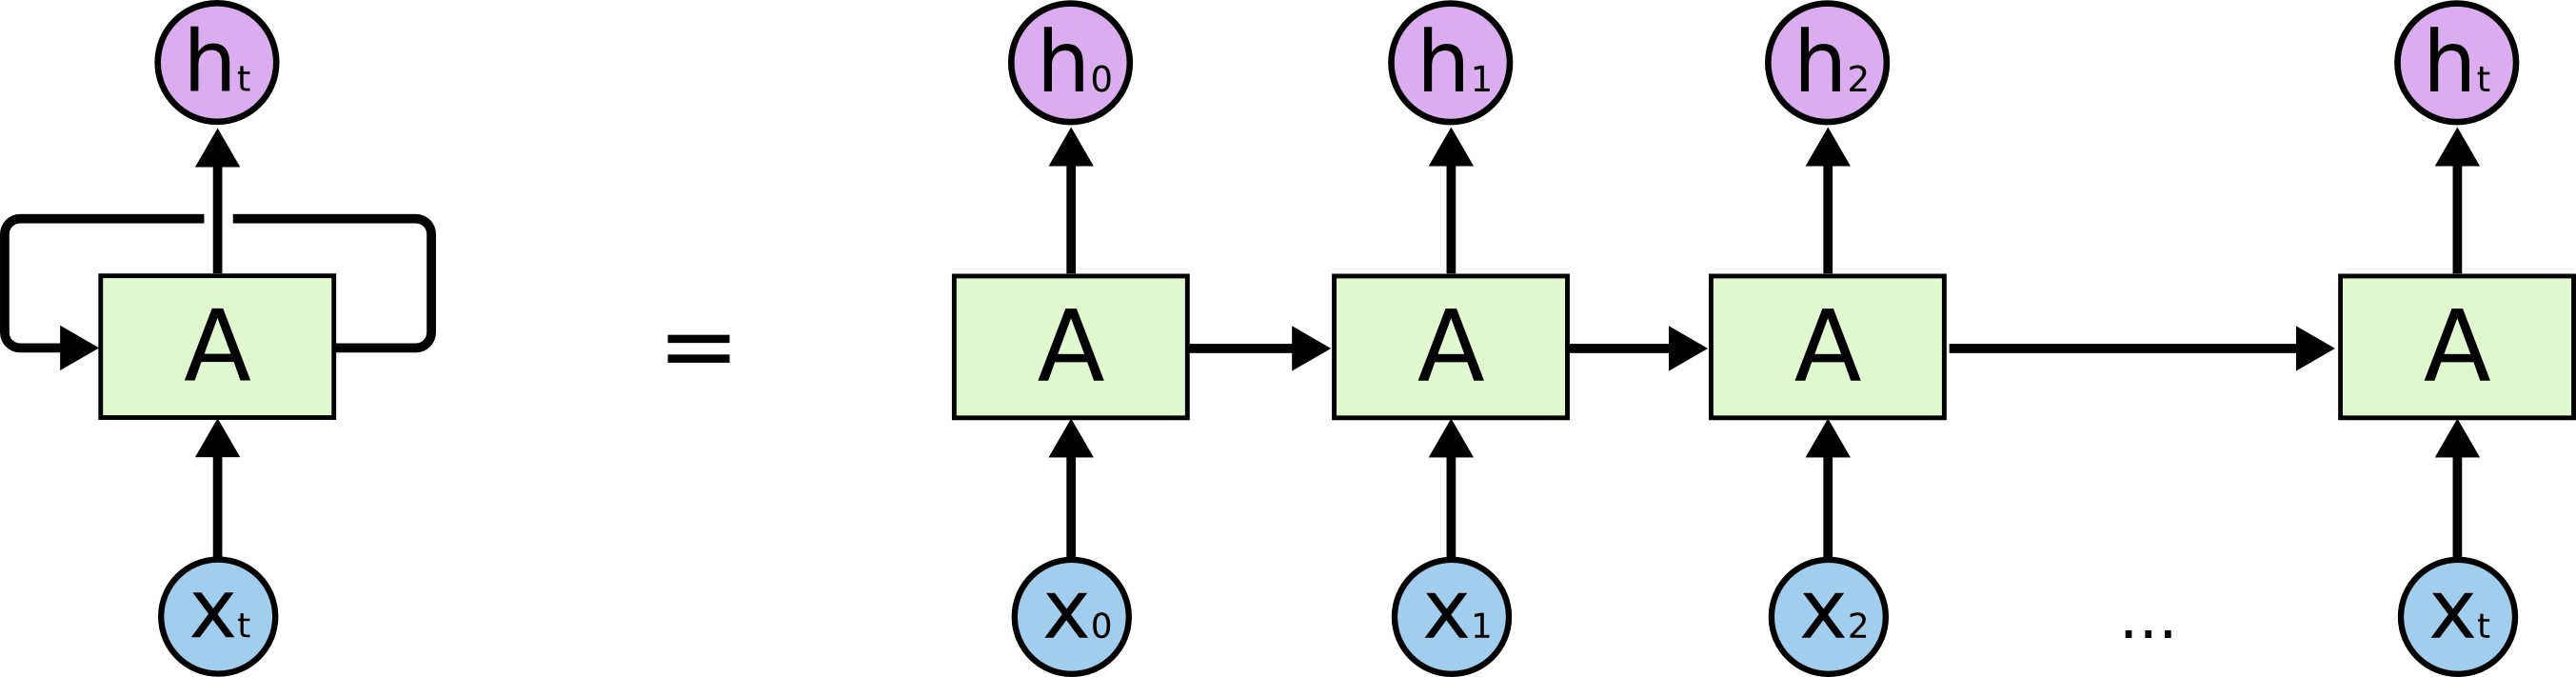
\includegraphics[width=1.0\textwidth]{RNN-unrolled.png}
  \end{figure}
\end{frame}

\begin{frame}[fragile]{网络架构}
  \begin{figure}
    \centering
    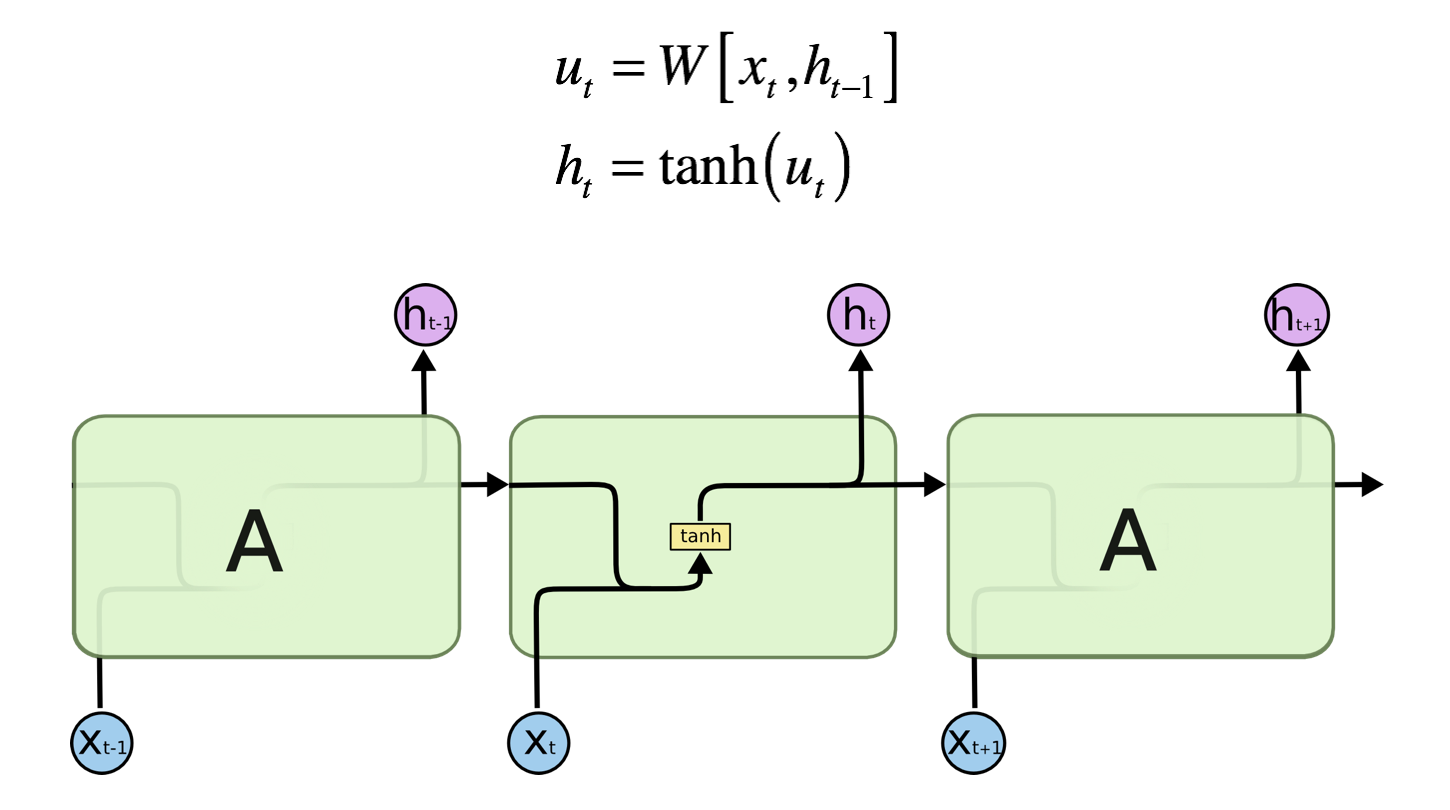
\includegraphics[width=1.0\textwidth]{LSTM3-SimpleRNN.png}
  \end{figure}
\end{frame}

\begin{frame}[fragile]{网络架构}
  \begin{figure}
    \centering
    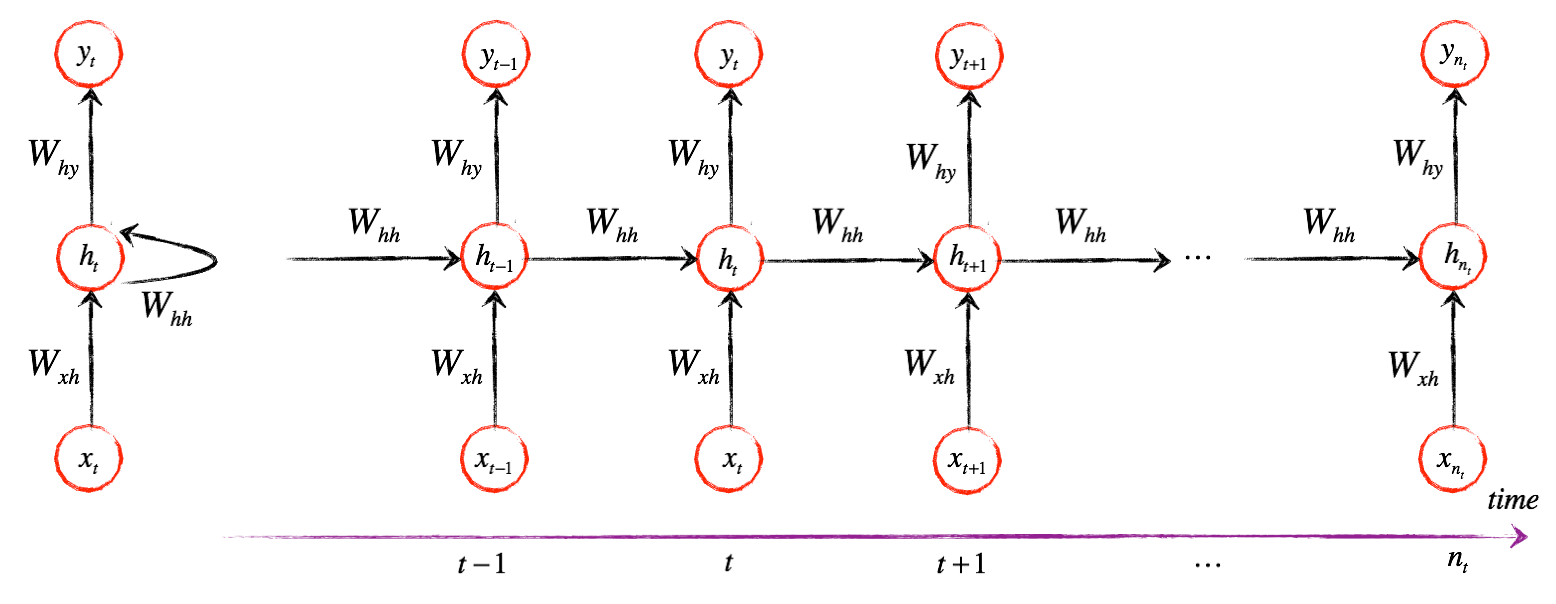
\includegraphics[width=1.0\textwidth]{rnn.png}
  \end{figure}
\end{frame}

\begin{frame}[fragile]{前向计算}
  \begin{figure}
    \centering
    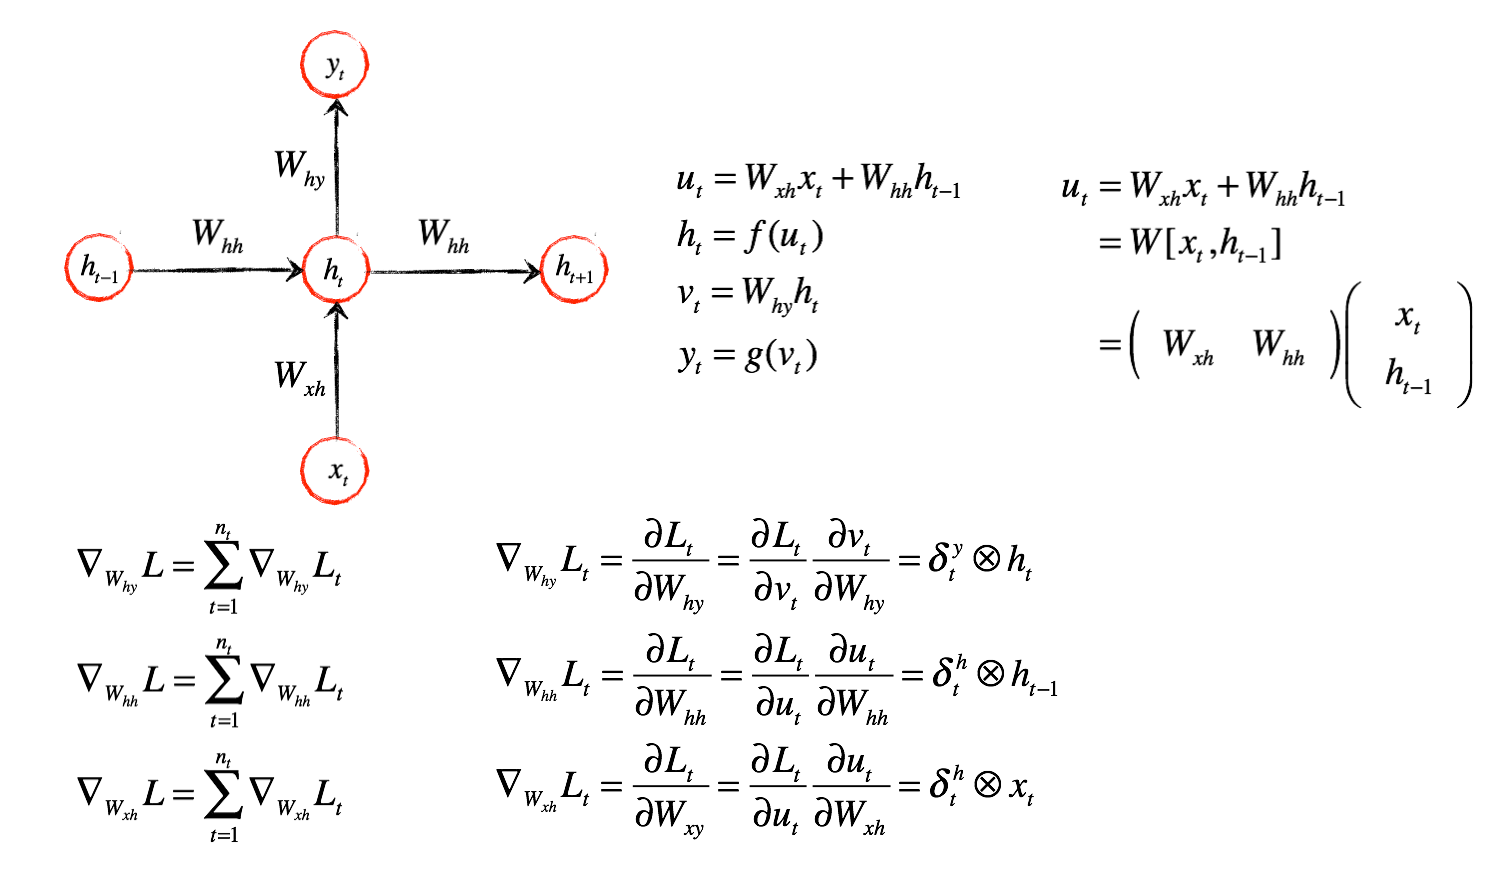
\includegraphics[width=0.9\textwidth]{rnn-fprog.png}
  \end{figure}
\end{frame}

\begin{frame}[fragile]{反向传播:BPTT}
  \begin{figure}
    \centering
    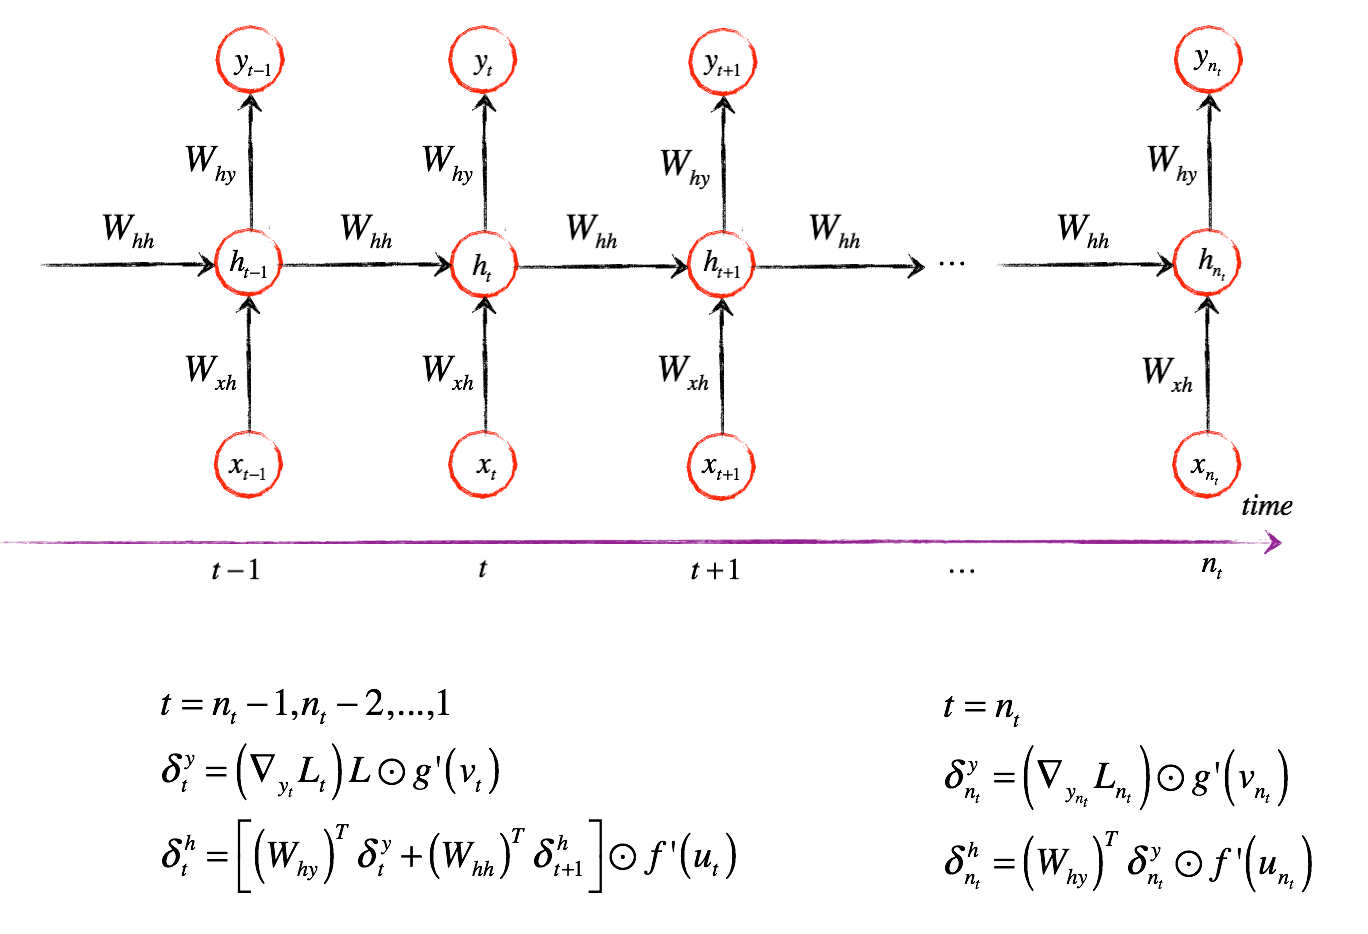
\includegraphics[width=0.85\textwidth]{rnn-bptt.png}
  \end{figure}
\end{frame}

\subsection{双向RNN}

\begin{frame}[fragile]{网络架构}
  \begin{figure}
    \centering
    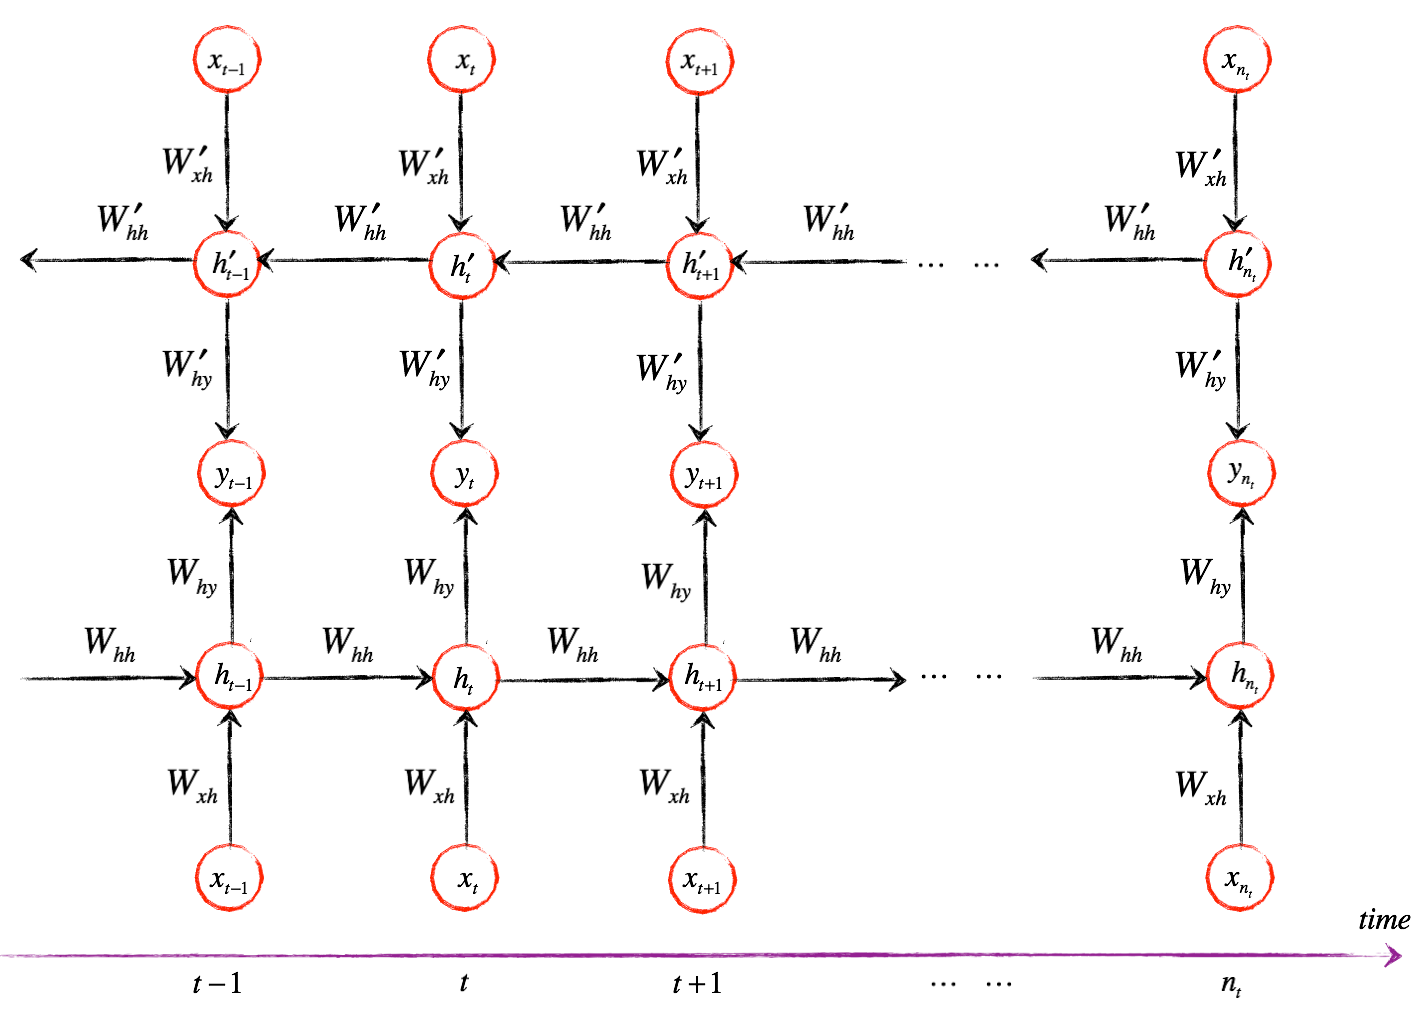
\includegraphics[width=0.8\textwidth]{drnn.png}
  \end{figure}
\end{frame}

\begin{frame}[fragile]{前向计算}
  \begin{figure}
    \centering
    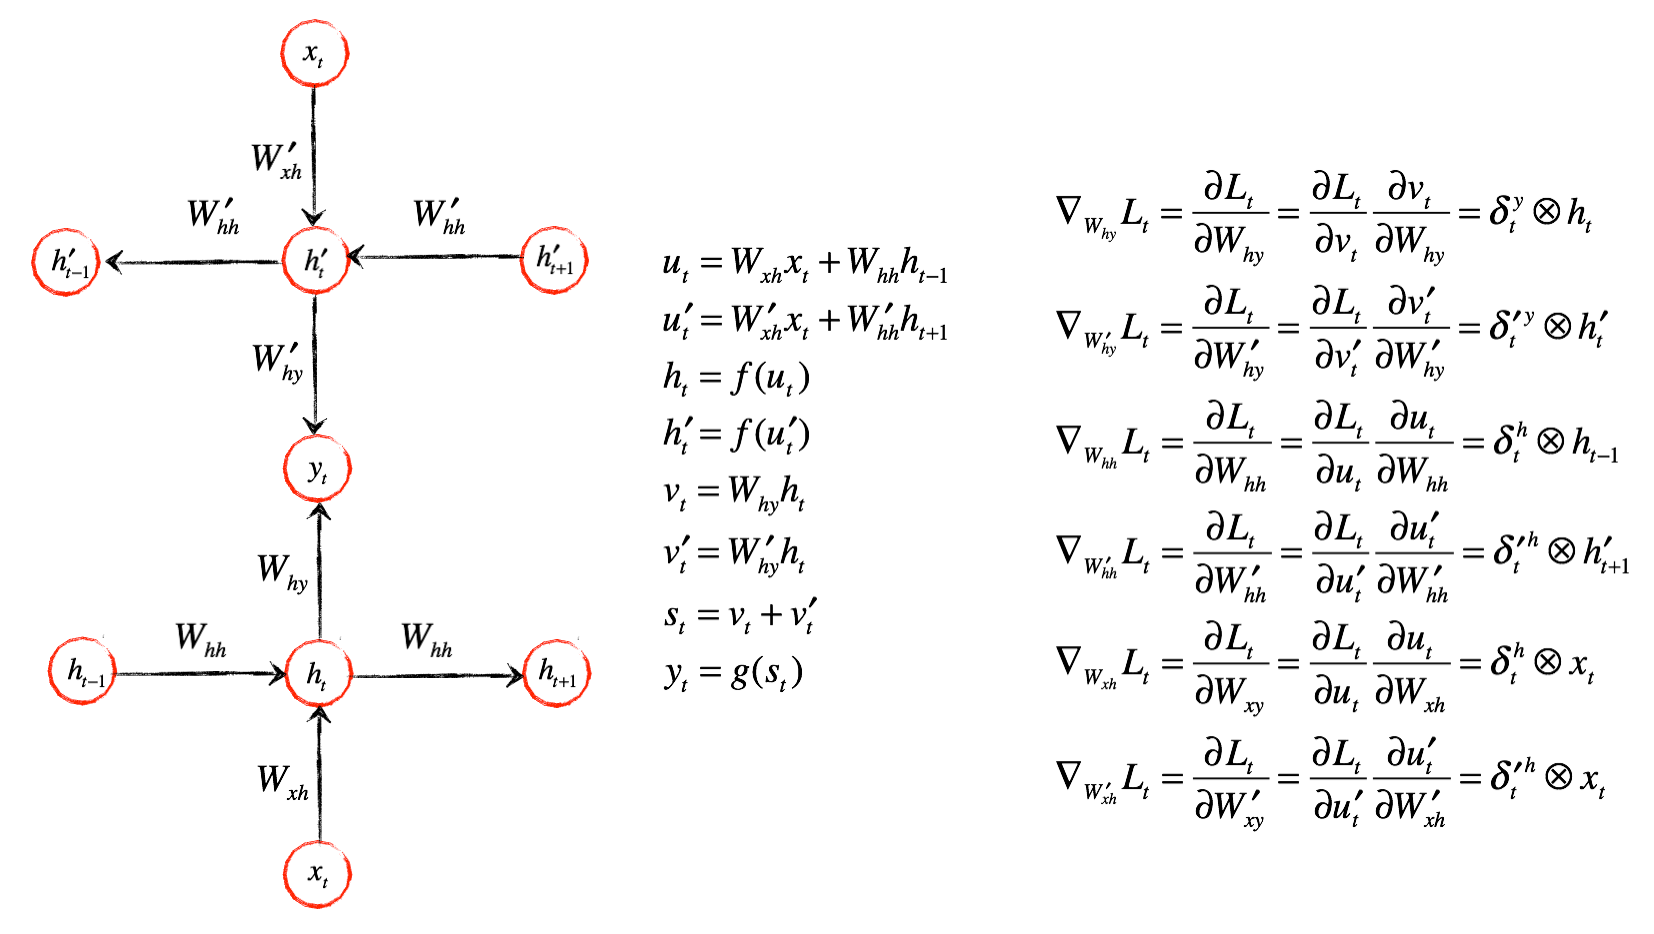
\includegraphics[width=1.0\textwidth]{drnn-fprog.png}
  \end{figure}
\end{frame}

\begin{frame}[fragile]{反向传播:BPTT}
  \begin{figure}
    \centering
    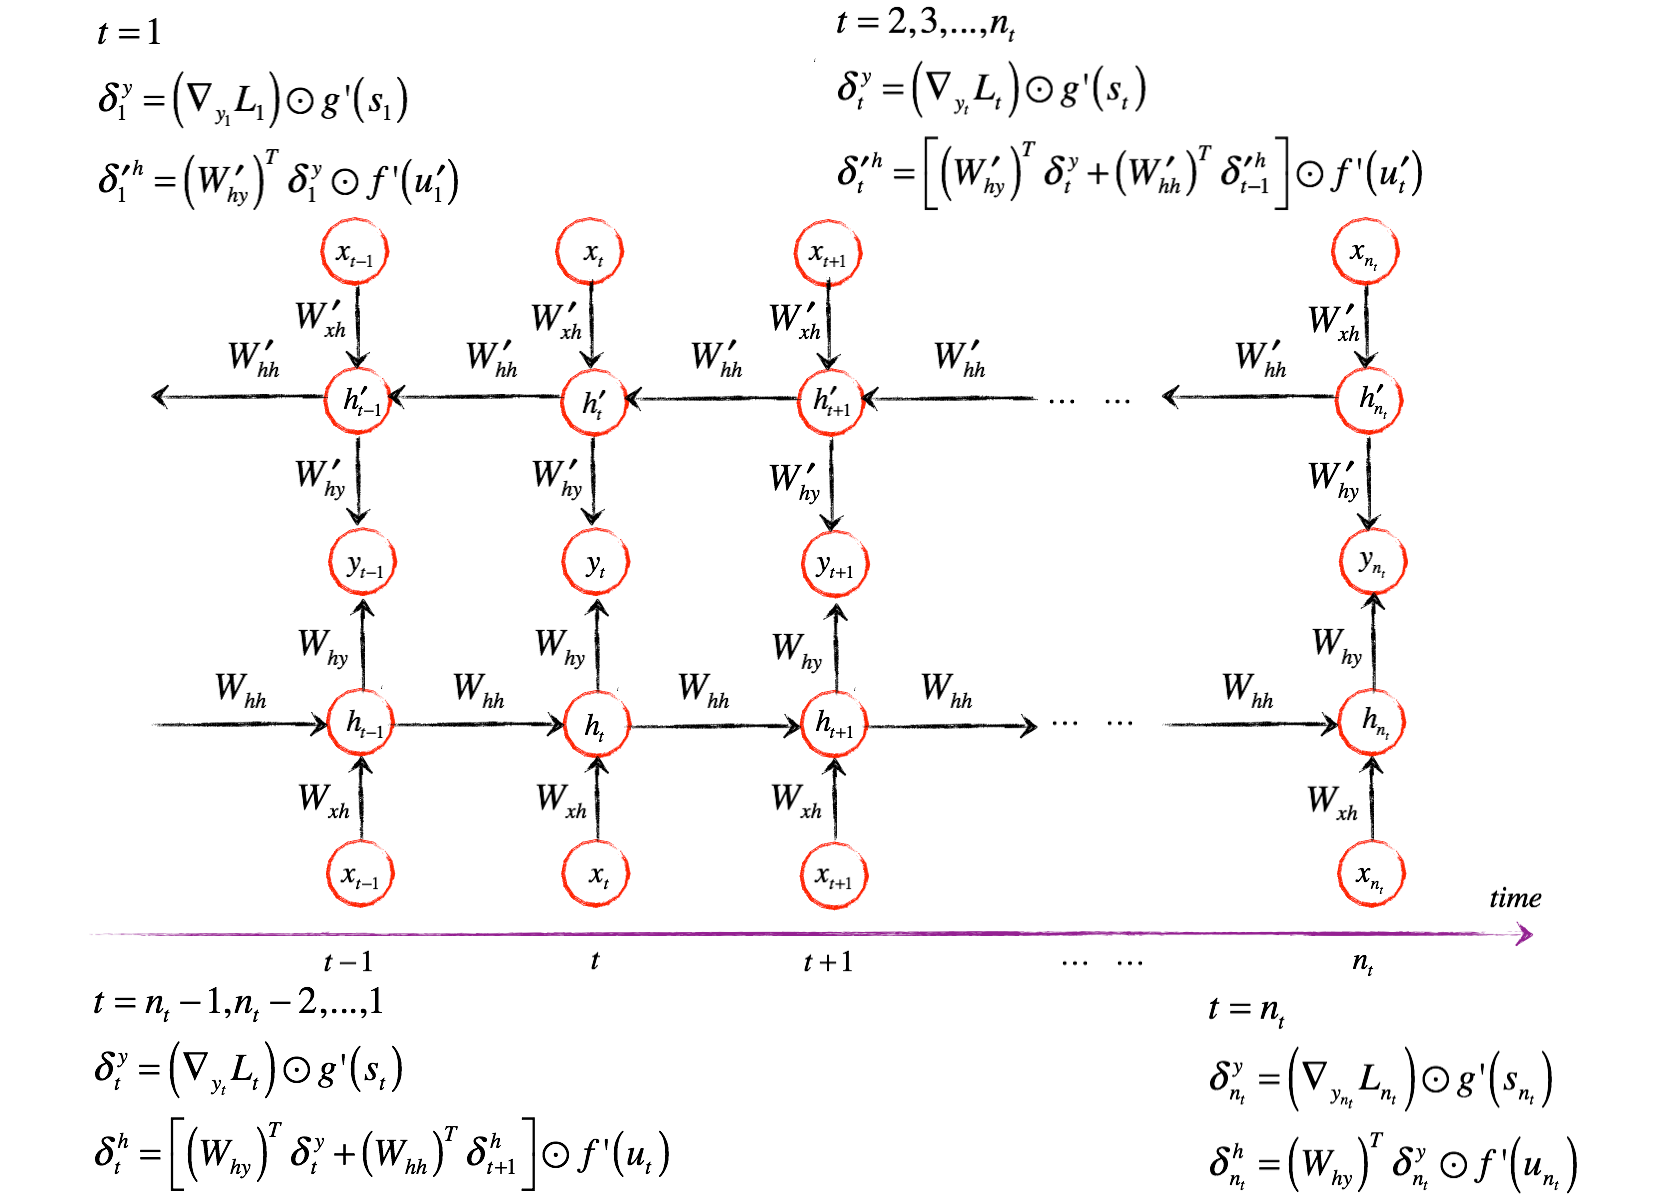
\includegraphics[width=0.75\textwidth]{drnn-bptt.png}
  \end{figure}
\end{frame}

\subsection{深层RNN}

\begin{frame}[fragile]{网络架构}
  \begin{figure}
    \centering
    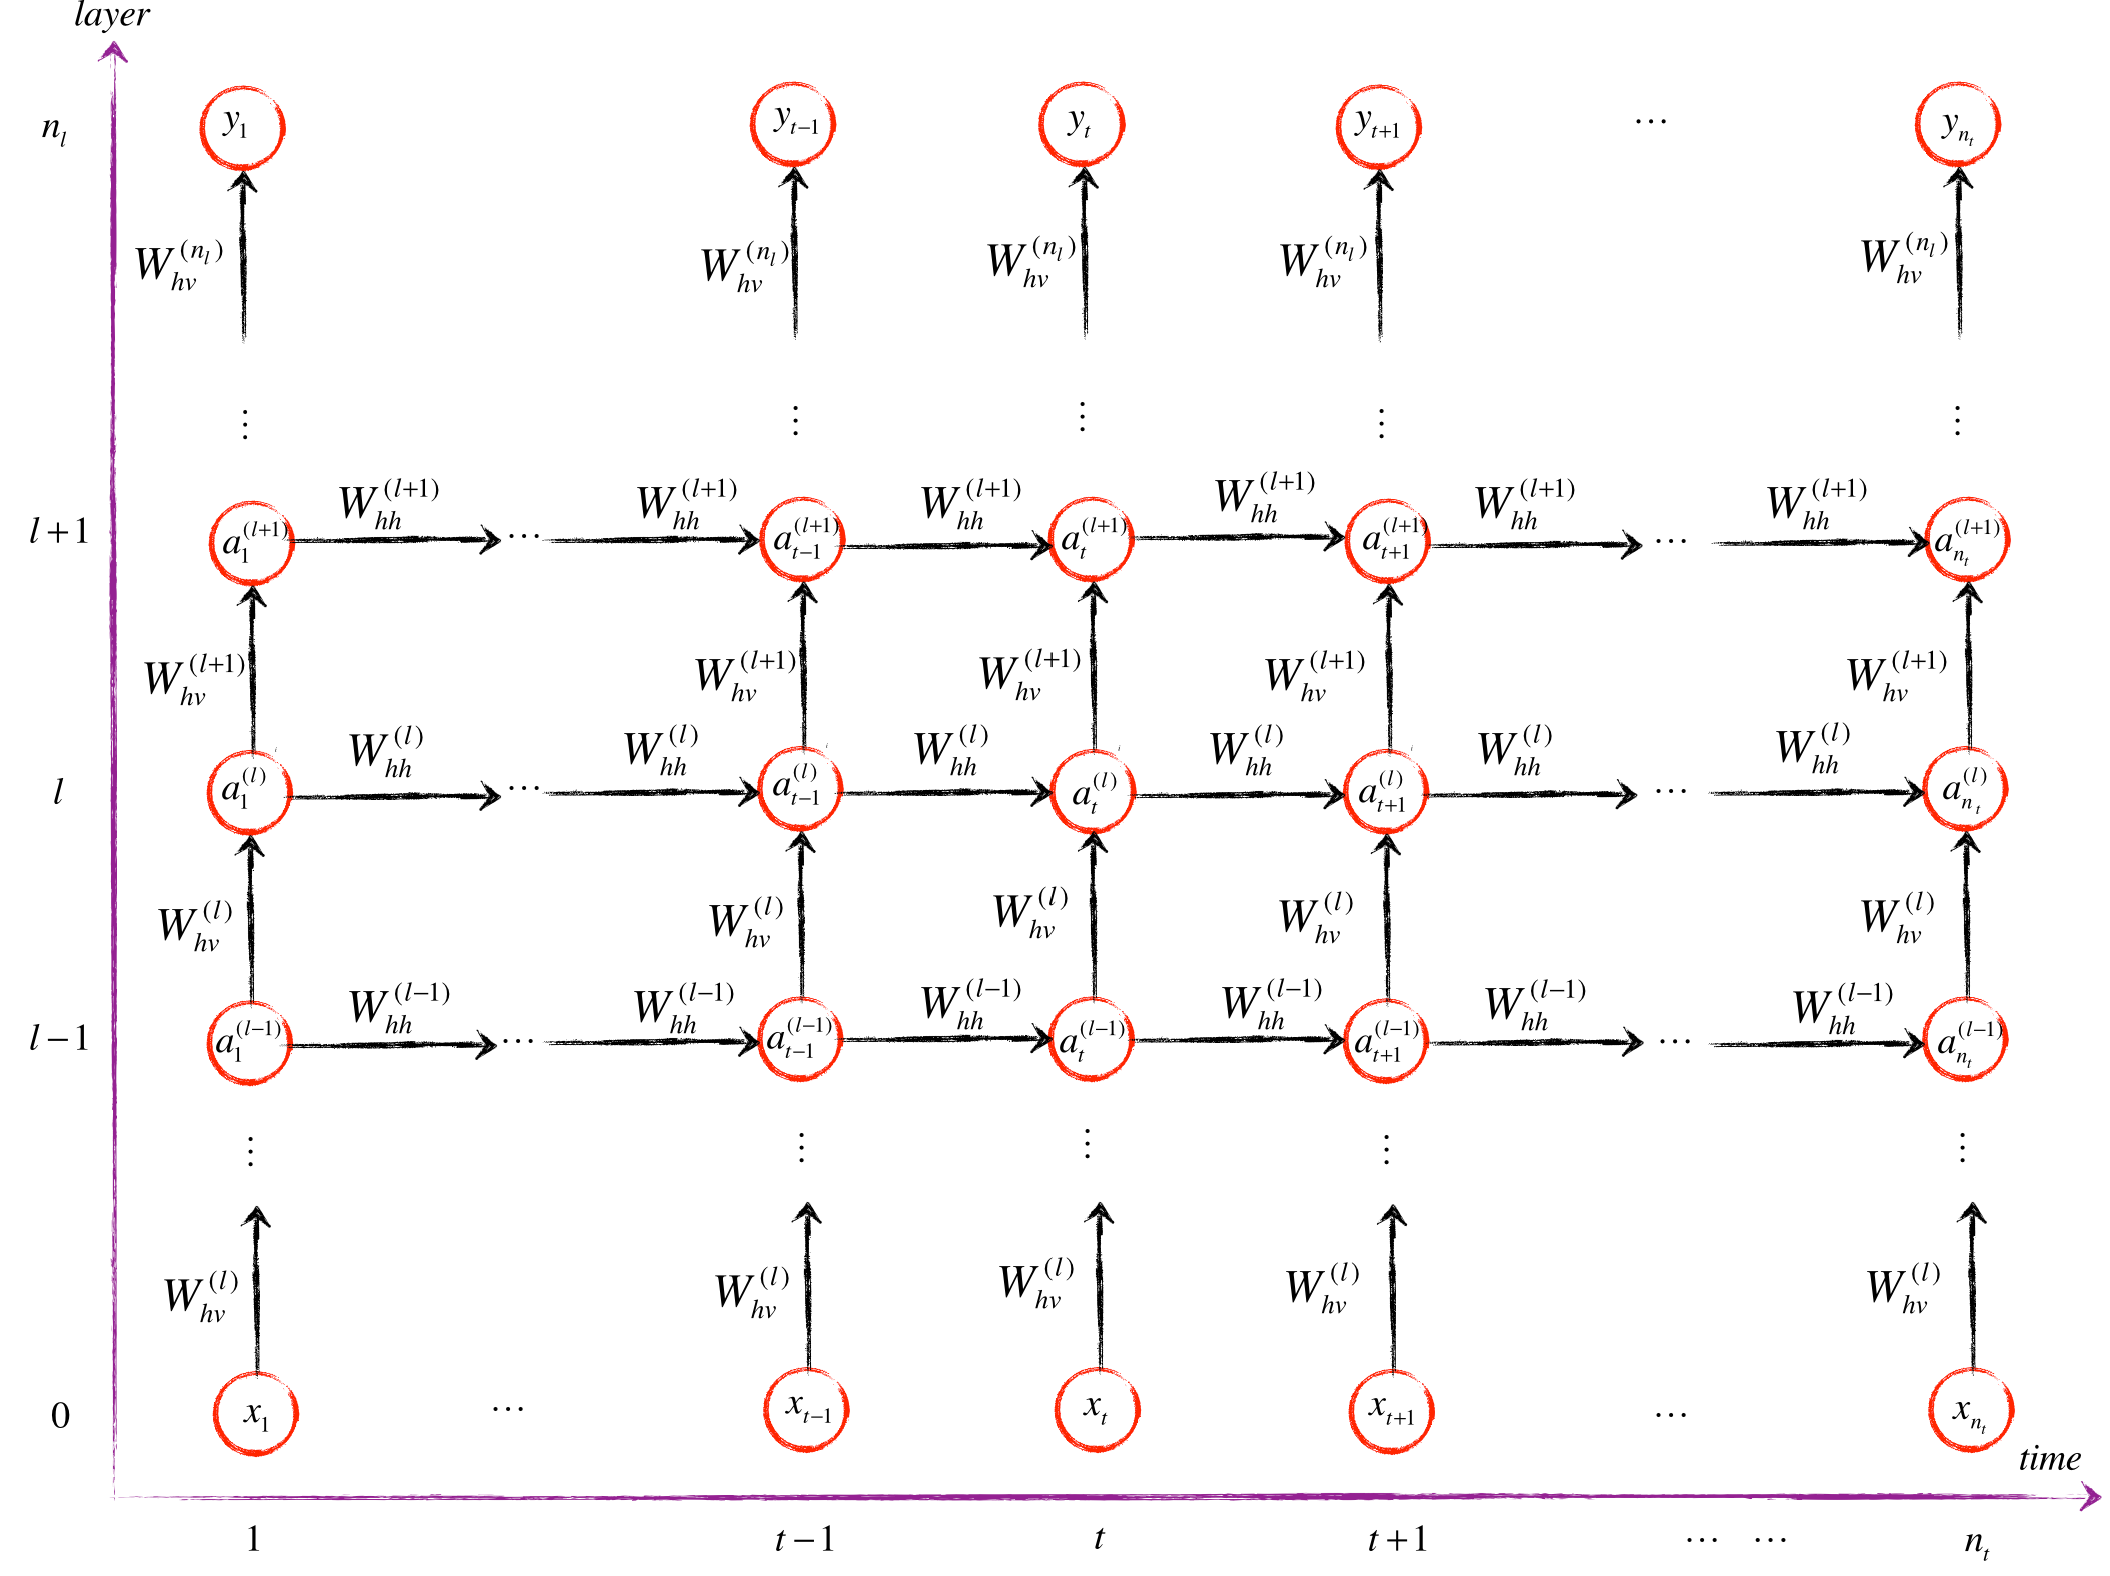
\includegraphics[width=0.8\textwidth]{dnn-rnn.png}
  \end{figure}
\end{frame}

\begin{frame}[fragile]{前向计算}
  \begin{figure}
    \centering
    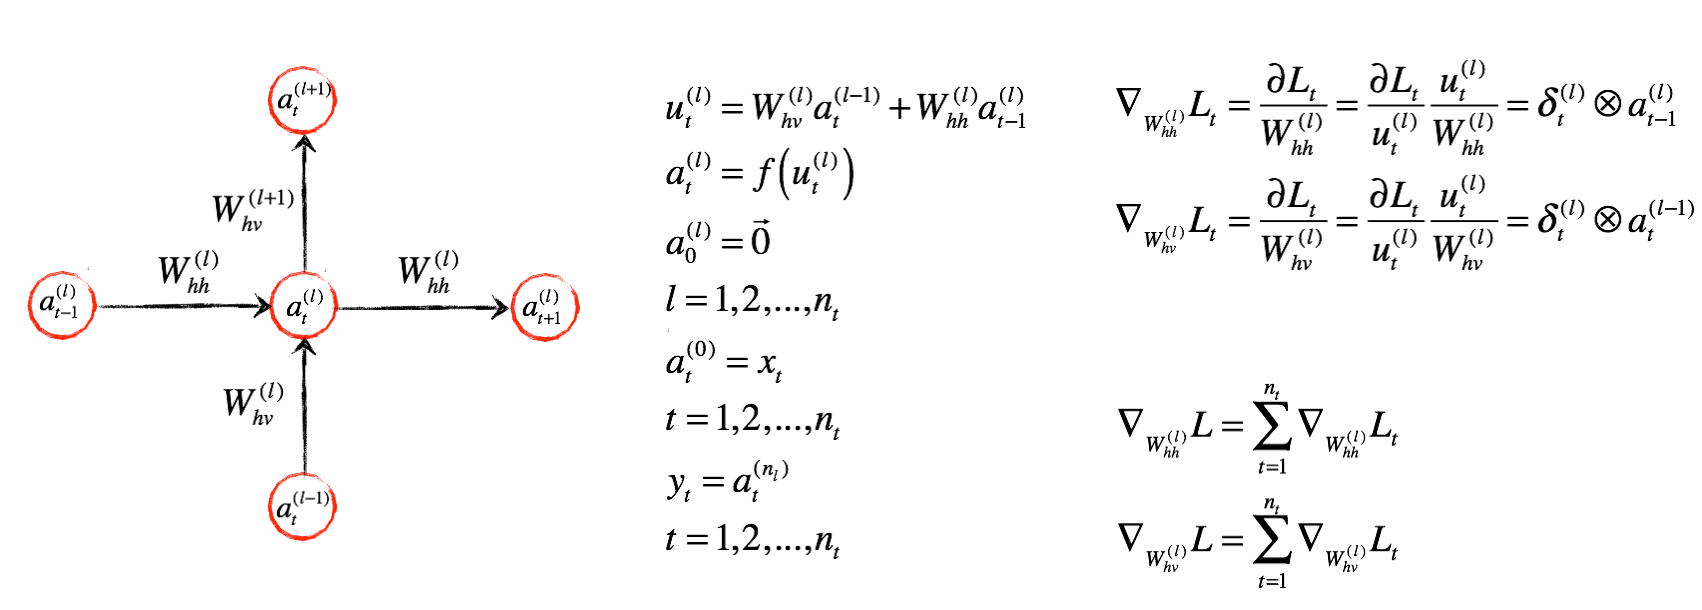
\includegraphics[width=1.0\textwidth]{dnn-rnn-fprog.png}
  \end{figure}
\end{frame}

\begin{frame}[fragile]{反向传播:BPTT}
  \begin{figure}
    \centering
    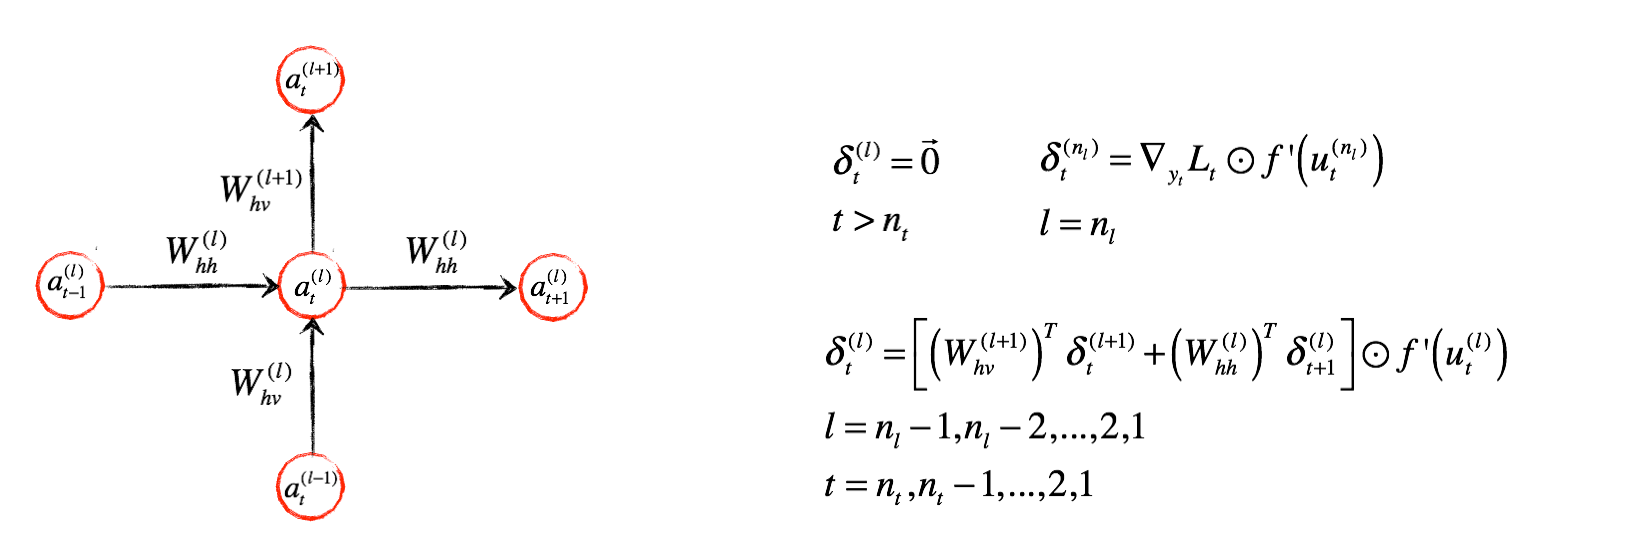
\includegraphics[width=1.0\textwidth]{dnn-rnn-bptt.png}
  \end{figure}
\end{frame}

